\documentclass[UTF8]{article}
\usepackage[UTF8]{ctex}
\usepackage[a4paper, margin=1in]{geometry}
\usepackage{amsmath}
% \usepackage{extramarks} % Required for headers and footers
\usepackage{fancyhdr} % Required for custom headers
\usepackage{lastpage} % Required to determine the last page for the footer
\usepackage{graphicx} % Required to insert images


\cfoot{第\ \thepage\ 页}

\large
\title{Homework-Chapter 2}
\begin{document}
\begin{titlepage}
    \begin{center}
        \line(1,0){300}\\
        [0.65cm]
        \huge{\bfseries Homework IV }\\
        \line(1,0){300}\\
        \textsc{\Large WireShark Intr}\\
        \textnormal{\Large \today}\\
        [5.5cm]
    \end{center}
    \begin{flushright}
        \texttt{\Large 谢远峰\\网安一班\\3019244283}\\
        [0.5cm]
    \end{flushright}
\end{titlepage}
\clearpage
\section*{Question 1}
List 3 different protocols that appear in the protocol column in the unfiltered packet-listing window in step 7 above. \par
ARP、DNS、TLSV1.2\par
\section*{Question 2}
How long did it take from when the HTTP GET message was sent until the HTTP OK reply was received?\par
大约0.2s\par
\section*{Question 3}
What is the Internet address of the gaia.cs.umass.edu?What is the Internet address of your computer?\par
网站的地址为128.119.245.12,个人电脑的地址为172.23.246.131\par
\section*{Question 4}
\begin{figure}[h]
    \centering
    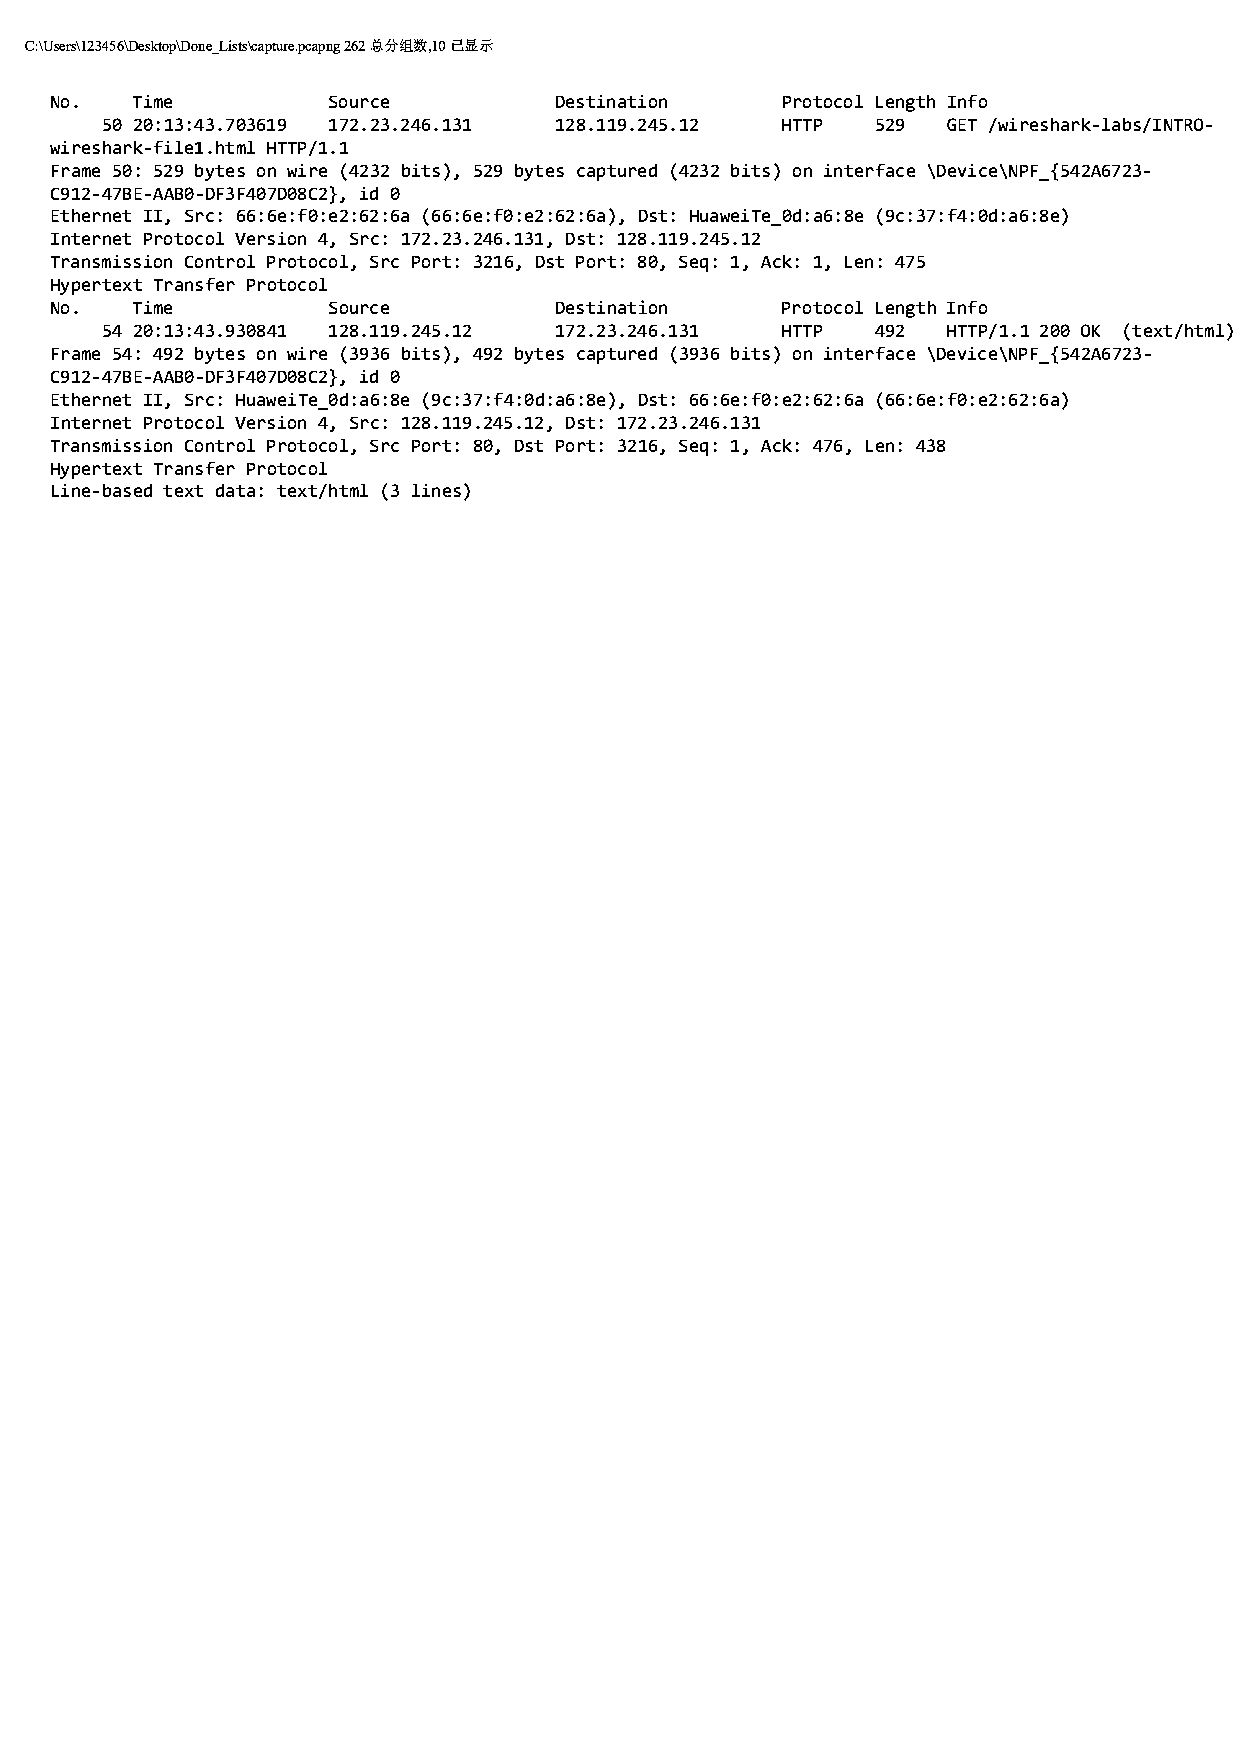
\includegraphics[width=16cm,height=8cm]{capture.pdf}
    \caption{HTTP-Messages}
\end{figure}
在几次静态页面的刷新后,浏览器注意到页面内容并未发生改变,其网络状态码为304。得知在对某一个服务器发出连续的HTTP请求时,如果服务器检查资源没有被修改就回复304 Not Modified,直接从本地缓存中调出数据,方便快捷。
\end{document}